\chapter{\LaTeX{} 基础}

\section{字符}

字符是文档最基本元素。
最基础的 \TeX{}/\LaTeX{} 系统仅支持英文,我们就先从英文排版说起。
不同于 Word 中任何一个用键盘输入的字符都可以直接显示出来,
\LaTeX{} 作为一种排版语言,不可能把任何一个字符都仅当作输出字符处理,
而是需要占用一些字符,来表达指令,帮助系统完成排版的任务。
这些字符是不能直接输出的。
此外,如果这些字符不合时宜地出现在正文里,还会引起错误。
这些字符有
\begin{center}
  \begin{tabular}{llll}
    \verb|%| & 注释符 & \qquad \verb|\| & 命令前导符 \\
    \verb|^| & 上标符 & \qquad \verb|$| & 数学模式符 \\
    \verb|_| & 下标符 & \qquad \verb|#| & 参数表达符 \\
    \verb|~| & 空格符 & \qquad \verb|{| & 参数起始符 \\
    \verb|&| & 分列符 & \qquad \verb|}| & 参数结束符 \\
  \end{tabular}
\end{center}
如果你希望这些字符可以在正文中显示,
“\textbackslash”符号可以用 \verb|\textbackslash| 显示,
其他符号都可以用 \verb|\符号{}| 的方式来显示,
如“\{”可以通过输入 \verb|\{{}| 来显示。
但 \verb|\\{}| 不能用来输入“\textbackslash”,它是换行命令。


\section{命令}

\LaTeX{} 中,命令最基本的形式是
\begin{center}
  \verb|\命令[可选参数]{参数}|
\end{center}
其中 \verb|\| 起到引导命令的作用,
方括号内的参数是可选的,没有方括号可以使用默认参数,
花括号内的参数是必选的,对于定义了必选参数的命令,必须给出参数。

下面从最简单的看起。
就像上一节介绍怎样在正文中打印出字符,其实就是用简单的命令实现的。
其中的“\verb|{}|”并没有给出参数,因此它不是完全必要的,
但有些字符的打印,没有它无法通过编译,为了便于记忆,打印保留字符时不妨都加上。

再说说前面提到的换行命令 \verb|\\|,它还可写成带可选参数的形式。 \verb|\\[1em]|\\[1em]
方括号里的参数代表距离。
\LaTeX{} 中的距离单位有 \texttt{cm},\texttt{mm},\texttt{pt},\texttt{em} 等,
其中 \texttt{em} 表示一个字符的宽度。
效果嘛,你已经看到了。

\LaTeX{} 中还有一种特殊的成对出现的命令,它以下面的形式出现

{\small\vspace{-0.2em}%
\begin{verbatim}
              \begin{环境名}[可选参数]{必选参数}
                文字或命令
              \end{环境名}
\end{verbatim}}

\vspace{-0.6em}\noindent
利用环境可以实现各种更加复杂的排版效果,例如列表和浮动的图表等。

最后,试试命令 \verb|\LaTeX{}| 吧。


\section{文档的基本结构}

最基本的 \LaTeX{} 文档实现形式如下

{\small\vspace{-0.2em}%
\begin{verbatim}
              \documentclass[参数]{article}
                导言区
              \begin{document}
                正文
              \end{document}
\end{verbatim}}

\vspace{-0.6em}\noindent
其中 \texttt{article} 可以用其他文类代替,
输入特定参数则可以实现特殊的排版效果。

导言区内可以利用命令 \verb|\usepackage[参数]{宏包}| 来实现各种复杂的功能,
或者自定义命令,满足自己写文章时特殊的需求。如输入一个公式
\verb|$$ \int\sin x\,d x $$| $$ \int\sin x\,d x $$
其中 $d$ 是微分算符,应该写成正体,可以用命令 \verb|\textrm{d}| 实现。
于是我们输入 \verb|$$ \int\sin x\,\textrm{d} x $$|
得到 $$ \int\sin x\,\textrm{d} x $$
但每次都这样输入是在麻烦,我们只需要在导言区做这样的定义
\begin{center}
  \verb|\newcommand{\diff}{\textrm{d}}|
\end{center}
这样,我们输入 \verb|$$ \int\sin x\,\diff x $$| 也能达到一样的效果。
对于某些高频率的比较复杂的输入,这样的自定义命令是不是会给你带来很大的便利呢。

下面说说正文。正文部分可以输入文字、公式,可以插入图表,
还可以利用各种命令和环境来实现特定的排版效果。
首先,要了解的是 \LaTeX{} 正文排版规则。
不同于 Word 利用软回车换行,用硬回车分段,连续的空格可以增加横向的间距。
\LaTeX{} 中回车和空格都自动产生一个空格以分隔单词。
连续的空格并不能在输出上产生更多的横向间距。
例如这段话,它的源代码如下。

{\small%\vspace{-0.8em}%
\begin{verbatim}
         下面说说正文。正文部分可以输入文字、公式,可以插入图表,
         还可以利用各种命令和环境来实现特定的排版效果。
         首先,要了解的是 \LaTeX{} 正文排版规则。
         不同于 Word 利用软回车换行,用硬回车分段,
         连续的空格可以增加横向的间距。
         \LaTeX{} 中回车和空格都自动产生一个空格以分隔单词。
         连续的空格并不能在输出上产生更多的横向间距。
         例如这段话,它的源代码如下。
\end{verbatim}}

前面我们已经知道了换行命令,那么 \LaTeX{} 中如何产生新的一段呢?
只要本段内容与上一段内容间有空白行(仅有空格,制表符或者字符),
\LaTeX{} 就会开起新的段落。
与空格同样,更多的回车也不能增加段落的间距。


\section{标题与文档逻辑结构}

\LaTeX{} 最大的特点就是你主要注意文章的逻辑结构。
即告诉 \LaTeX{} 什么地方新起一章,什么时候新起一节,
\LaTeX{} 会自动给各个章节标题编号并套用相应的格式。
一般而言,作者无需关心章节标题格式的问题,
但有时为了满足特定的需求,通过一些宏包,也可以修改章节标题的格式。
大多科学杂志出版社要求使用 \LaTeX{} 格式的文档投稿,
最大的优势就在于可以地方便套用预设的模板达到出版社所需的排版效果,
而无需对正文的内容作其他的调整。

首先介绍文章标题。
\LaTeX{} 可自动生成标题。
在导言区或正文开头用命令
\begin{center}
  \verb|\title{{标题}}|,\verb|\author{作者}| 和 \verb|\date{日期}|
\end{center}
可以对标题的要素进行申明,而后用命令
\begin{center}
  \verb|\maketitle|
\end{center}
就可以自动生成格式优美的标题了。
需要说明的是,如果不需要打印作者,可以略去对作者的声明,
但如果略去对时间的什么,则会打印出当前日期。
如果不需要打印日期,则要这样声明: \verb|\date{}|。

正文中,开起新的章节的命令分别是
\begin{center}
  \verb|\chapter{章标题}| 和 \verb|\section{节标题}|
\end{center}
同时,还可以用
\verb|\subsection{标题}| 和 \verb|\subsubsection{标题}|
来开起更细的标题结构。
需要注意的是,\texttt{article} 文类是没有章标题的,它一般比较适合排版短篇论文。
对于长篇报告和书籍,需要使用文类 \texttt{report} 和 \texttt{book}。

同时,文章中有时候还需要用到罗列环境。
罗列环境有常用和排序两种。
常用罗列环境的形式和排版效果如下

\vspace{1.2em}
\begin{minipage}{0.5\textwidth}
\small
\begin{verbatim}
      \begin{itemize}
        \item 条目1
        \item 条目2
        \item[**] 条目3
      \end{itemize}
\end{verbatim}
\end{minipage}\qquad\begin{minipage}{0.3\textwidth}
\begin{itemize}
  \item 条目1
  \item 条目2
  \item[**] 条目3
\end{itemize}
\end{minipage}

\vspace{1.2em}\noindent
常用罗列环境的形式和排版效果如下

\vspace{1.2em}
\begin{minipage}{0.5\textwidth}
\small
\begin{verbatim}
      \begin{enumerate}
        \item 条目1
        \item 条目2
        \item[**] 条目3
      \end{enumerate}
\end{verbatim}
\end{minipage}\qquad\begin{minipage}{0.3\textwidth}
\begin{enumerate}
  \item 条目1
  \item 条目2
  \item[**] 条目3
\end{enumerate}
\end{minipage}

\vspace{1.2em}\noindent
罗列环境还可以嵌套使用。

最后说一下中文排版。
中文排版只需要将 \LaTeX{} 预置的三种文类 
\texttt{article},\texttt{report} 和 \texttt{book}
替换为 \texttt{ctexart},\texttt{ctexrep} 和 \texttt{ctexbook} 即可。
中英文混排中,需要注意的一个细节是中英之间的空格。
英文中把回车和空格都当作一个空格处理。
这样处理,显然不符合中文的排版习惯,因为汉字不像单词,之间是不会出现空格的。
而这种情况下,源文件换行必定会在输出上出现不必要的空格。
用 LaTeX 或 pdfLaTeX 编译时,一般有两种解决方案。
一种是依旧把回车和空格当作空格处理,
在每一行末尾加上 \verb|%| 以注释掉回车。
这显然过于繁琐了。
另一种是让编译器忽略掉中文字符间的空格,
这时系统也会自动把中文和英文之间的空格忽略掉。
(英文单词之间的空格还是会保留)
一般我们在中文和英文之间需要插入一个 \verb|~| 符号产生一个小空格,排版效果才比较好。
这又是我推荐使用 XeLaTeX 进行编译的另一个重要原因。
编译器会自动处理这些空格,
而无需对行末的回车进行注释或是在中文和英文单词间加入额外的空格,就能得到理想的排版效果。
但我仍习惯在中文和英文之间键入一个空格,不过键入空格可比键入 \verb|~| 方便得多。

至此,纯文字的排版基本上就介绍完了。


\section{公式}

前面多次提到 \LaTeX{} 比起 Word 很大的一个优势,就是它的公式输入和排版。
先说说它的排版效果吧。
\LaTeX{} 非常智能,对于出现在文字中的公式(行内公式)和单独占用一行的公式(行间公式)
可以自动作出调整。
用 Word 写文档一般要求用 Mathtype 插入公式,
插入行内公式,哪怕只是 $x$, $y$, $z$ 这样的变量,也会引起行间距增加,
使排版效果大打折扣。
如果插入 $\frac{1}{x}$ 这样的分式,那排版的效果简直就 undirectlookable 了。
下面给大家看一下,同样一段话用 Word 排版的效果。

\begin{figure}[htb]
\vspace{0.6em}
\begin{center}
  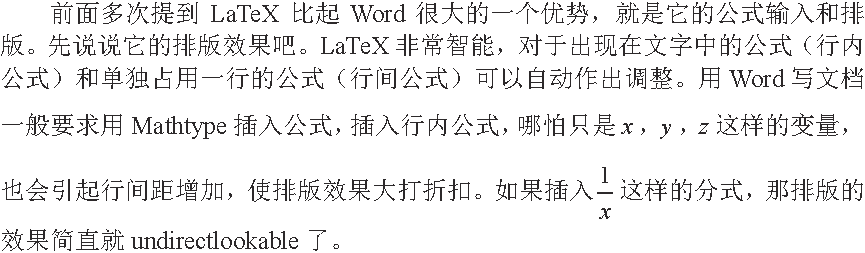
\includegraphics[width=0.9\textwidth]{fortest/wordexample}
\end{center}
\vspace{-1em}
\end{figure}

下面说说在 \LaTeX{} 如何输入公式。
虽然 \LaTeX{} 的公式输入都是靠代码实现,
但 \LaTeX{} 输入公式的语法非常简单,
甚至可以说,以英文为母语的人只要会读,就可以把公式写出来。
先看看下面这个公式
$$  \int_{-1}^{1} \frac{f(x)}{\sqrt{1-x^2}}\,\mathrm{d}x
   =\frac{\pi}{n}\sum_{k=1}^{n}f\left(\cos\frac{2k-1}{2n}\pi\right)
   +\frac{\pi}{2^{2n-1}(2n)!}f^{2n}(\theta) $$
看起来有点小复杂吧。
别急,只要稍加说明,打出比这更复杂的公式都是很简单的事情。

首先,需要学会开始一个公式。
最基础的 \LaTeX{} 中,要输入行内公式,应该这样做 \verb|$行内公式$|。
如果公式比较重要,或者形式比较复杂,
则一般写成行间公式的形式 $$\verb|$$行间公式$$|$$
前面出现的公式就是一个行间公式,我们也可以把它改写成行内公式的形式,效果是这样的
$  \int_{-1}^{1} \frac{f(x)}{\sqrt{1-x^2}}\,\mathrm{d}x
  =\frac{\pi}{n}\sum_{k=1}^{n}f\left(\cos\frac{2k-1}{2n}\pi\right)
  +\frac{\pi}{2^{2n-1}(2n)!}f^{2n}(\theta) $。
与其行间公式形式比较,\LaTeX{} 自动调整了字体大小,
并将求和上下限的位置改写到求和符号的右边以减小竖直方向的空间占用,保持行距。
虽然这样复杂的公式很少有人将它写成行内形式,
但也可以想象一下在 Word 里插入这样复杂的行内公式,
排版效果会变得多么糟糕。

学会了开始公式,我们学习最简单的表达式。
数字和变量直接输入就行,例如 \verb|$2x$| 就可以输出 $2x$ 了。
希腊字母怎么读就怎么输,\verb|$\alpha\beta\gamma$|
就可以输出 $\alpha\beta\gamma$ 了。
大写字母只要开头大写就行,输入 \verb|$\Delta\Phi\Psi$|
就能输出 $\Delta\Phi\Psi$。
等等,还有个小问题,有些字母是有变体的,需要在命令前加 \verb|var|。
如输入 \verb|$\varepsilon\varphi\varPhi\varPsi$|
就得到了 $\varepsilon\varphi\varPhi\varPsi$。
还有各种算符,算符需要用数学正体表示,以区别于变量。
\LaTeX{} 已经定义了很多算符命令,比如 \verb|$\lim,\ln,\sin,\cos$|
得到输出 $\lim,\ln,\sin,\cos$。
还有积分符号\linebreak $\int$:\verb|$\int$|,求和符号 $\sum$:\verb|$\sum$| 等,
别忘还有了我们前面自定义的微分算子 $\diff$:\verb|$\diff$|。
现在你应该能理解前面输入的命令 \verb|$\int\sin x\,\diff x$|
是怎样被翻译成公式 $\int\sin x\,\diff x$ 的了吧?
等等 \verb|\,| 是做什么的?
忘了说了,数学模式下空格是被自动忽略的,
输入 \verb|\,| 让 $\sin x$ 和 $\diff x$ 之间隔开一点
(具体说是六分之一空格),会比较好看哦,
如果没有它就变成了 $\int\sin x\diff x$, 是不是有点别扭呢。



